% 来源：OEBPS/Text/Section0001_split_002.xhtml#sigil_toc_id_16

\BookChapter{7}
\section[第7章\q 投资营销谎言2：“我们的收费？你付的只是小钱！”]{第7章\\ 投资营销谎言2：“我们的收费？你付的只是小钱！”}

\begin{BookQuote}
公募基金行业是全球最大的揩油机构，7万亿美元流进基金经理、经纪人和其他投资内行的手里，这可是美国很多家庭、院校、老人退休储蓄的钱。

\hfill ——彼得·菲茨杰拉德［参议员，2004年提出公募基金改革法案（后来让参议院银行委员会毙掉了）］
\end{BookQuote}


\subsection{先伤害，再侮辱}

再没有比这样的事更让人生气的了，告诉你的是一个价格，但是后来你发现你支付的是另外一个价格。你要买辆新车，谈好了价格，但是当你回去签合同的时候，就会有几千美元额外的费用神奇地冒出来。你住了一家酒店，退房结账时却发现要额外征收度假费、旅游税、无线上网费、毛巾使用费——你明白了吧。

这真让人沮丧。我们感觉让人骗了，被人暴力威胁，反正结果就是付的钱比我们本来应该付的多。借助使用极小号字体，资产规模高达13万亿美元的公募基金行业，轻松、熟练地隐藏了收费。

《福布斯》杂志刊登了一篇文章《持有公募基金的真正成本》，作者泰·伯尼克一层一层地揭开了各项费用，详细地分析了持有公募基金的真实成本，最后得出的结果简直让你心搏骤停：持有公募基金的平均成本是每年3.17\%！

3.17\%，听起来也不是什么大数字，你再回想一下我们前面了解到的东西，如果你持有指数基金，比较下二者的成本，你就明白了。例如，你可以拥有整个市场（比如拥有标准普尔500指数所有500只成分股），每年投资成本只有0.14\%，用投资界的行话来说就是14个基点。你投资100美元，只需要付0.14美元的费用。（你一学就会，马上就能听懂这个内行才知道的术语：100个基点就是1\%，50个基点就是0.5\%，以此类推。）

要拥有整个股市，只需要持有一只低成本指数基金，先锋公司和三维基金顾问公司都提供了这样的指数基金。我们已经知道持有指数基金，就可以拥有整个股市，长期业绩可以打败96\%的基金经理，尽管他们是专业的选股人。当然，你愿意支付3\%给非常厉害的对冲基金经理，就像瑞·达利欧，他从创立基金到现在每年的收益率高达21\%（扣费前）。对于大多数公募基金来说，我们支付的费用高了30倍，或者说高了3000\%，可是，我们得到的是什么呢？业绩还赶不上市场平均水平！你能想象吗？你买了一辆新车，和你邻居家的车一模一样，可你的价格却要高30倍，而且每小时只能跑25英里！

这就是现在投资主动管理型基金的现实情况。情况相同的两家人都把钱投资在股市上，一家每年要付大把的钱，但是另外一家投资1美元只需要付出几厘钱。

同样的收益率，不同的结果——无知的代价。

三个从小玩到大的好朋友，杰森、马太和泰勒，现在都35岁了，每个人都攒了10万美元来做投资，每个人分别选择了不同的基金。非常幸运的是，三个人获得的业绩相同，都是市场平均业绩，每年7\%。这样过了30年，他们65岁了，又聚到了一起，比比谁的投资账户里赚的钱更多。深入分析之后，他们发现三个人各自支付的费用差别很大。三个人每年支付的费用分别是1\%、2\%、3\%。

下面我们来算一算费用对他们最终积累财富的巨大影响：

杰森，本金10万美元，每年投资收益率7\%（扣掉每年3\%的费用），收益为324340美元；

马太，本金10万美元，每年投资收益率7\%（扣掉每年2\%的费用），收益为432194美元；

泰勒，本金10万美元，每年投资收益率7\%（扣掉每年1\%的费用），收益为574349美元。

同样的投资本金，同样的年化收益率，泰勒最后投资积累的财富接近他的朋友杰森的2倍。你会赌哪匹马赢呢？是那个100磅\footnote{\label{fn:pdf-7-1}1磅=0.4536千克。——编者注}重的马，还是那个300磅重的马？

\begin{figure}[htbp]
\centering
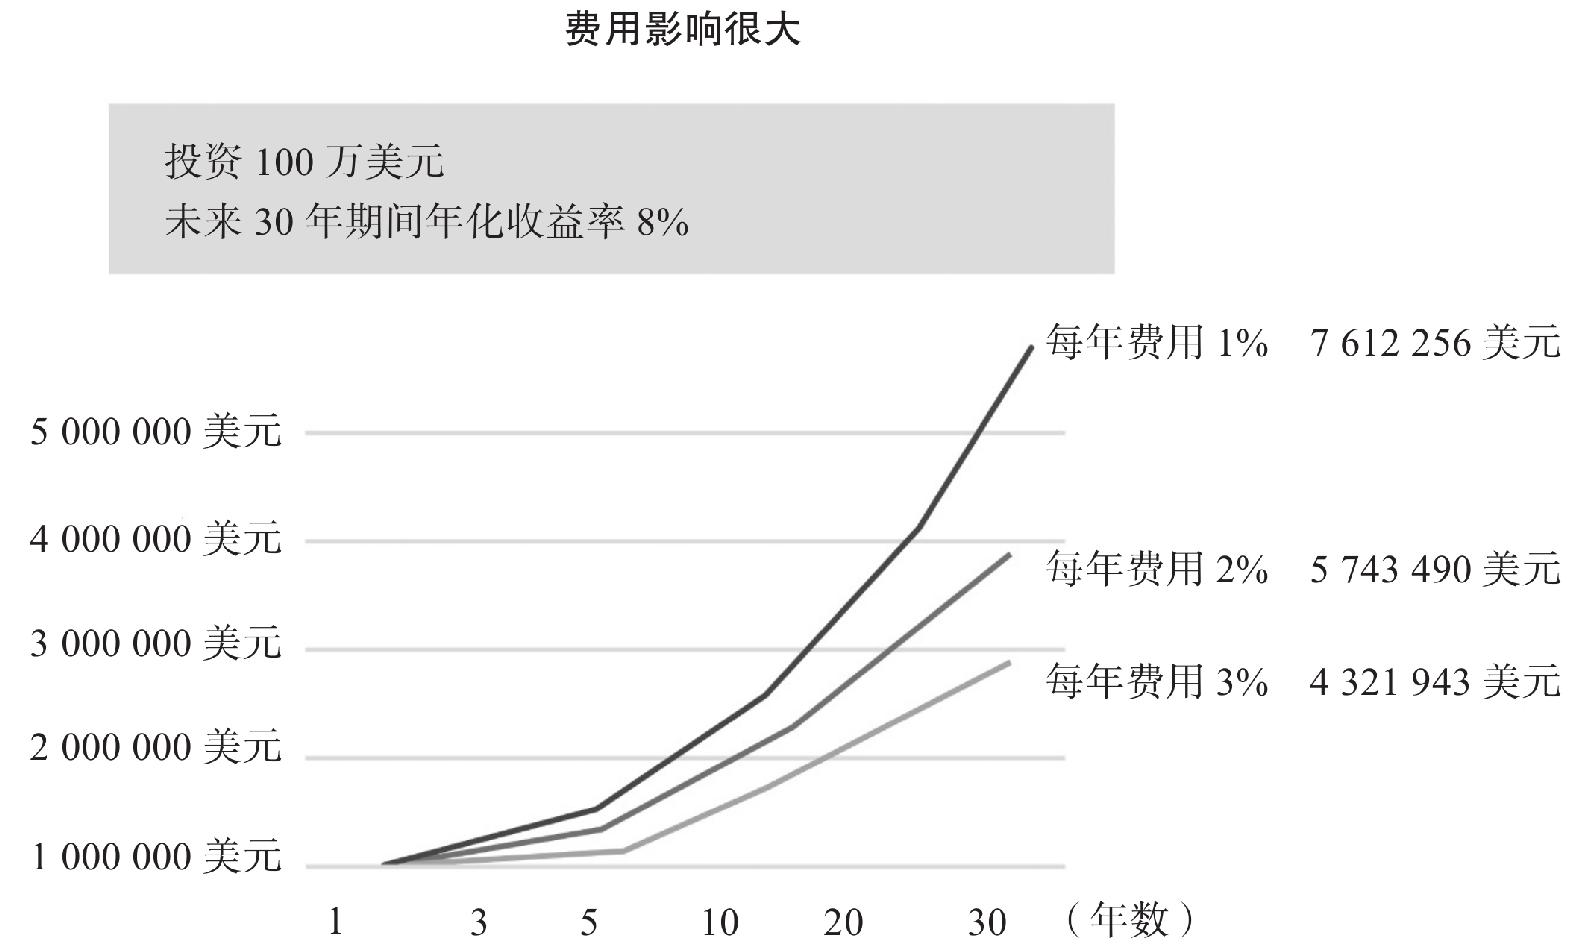
\includegraphics[width=0.86\linewidth,keepaspectratio]{image/7-1.jpg}
\caption{}\label{fig:7-1}
\end{figure}

“只不过”这里1\%，那里1\%而已，听起来好像没什么大不了的，但是在长期复利力量的作用下，这会造成巨大的差异，能决定你的一生能花的费用，政府能供养你多久，家庭给你的援助能持续多久。一种退休生活是一想到这个月的水、电、煤气账单都没钱付，就咬牙切齿；另一种是心平气和，过着自己想要的退休生活，享受着幸福的晚年。事实上，这也经常意味着退休时间会差别很大，一种是不得不再多工作十年，再赚点钱才够养老，另一种是我愿意就可以提前退休，因为养老金已经足够花了。正如约翰·博格教我们的那样，支付过高的费用相当于把你为未来攒的退休金送给别人50\%\textasciitilde{}70\%。

不过，上面举的例子只是假设，现在我们来看一下真实的情况。2000年1月1日—2012年12月31日，共有13个完整的年度，标准普尔500指数是平的，没有上涨，没有收益。这13个年度里面包括大家经常说的“失落的十年”，因为大多数人的投资根本没有任何回报，但是人们经受了巨大的振荡，2007年股市大涨，2008年却像自由落体一样暴跌，然后从2009年开始又出现一波大牛市。假如你把自己一辈子攒的10万美元投资到股市中，如果你只是持有整个股市或者说模拟整个市场，经过整整13年，你的投资账户是持平的，你的费用非常低，基本可以忽略。但是如果你买的是主动管理型公募基金，平均每年支付3.1\%的费用，假设你的公募基金经理还表现相当好，能够追平市场，也就是说基本持平、没有亏损，那么这13个年度你支付的费用就要超过3万美元！因此，你的投资账户上的资产还会少40\%，只剩下6万多美元，而市场持平，不涨也不跌。投资的资本金是你出的，风险是你承受的，而那些基金公司，不管出现什么情况，都照样赚钱，因为不管发生什么事情，它们都照样收取管理费。

\begin{figure}[htbp]
\centering
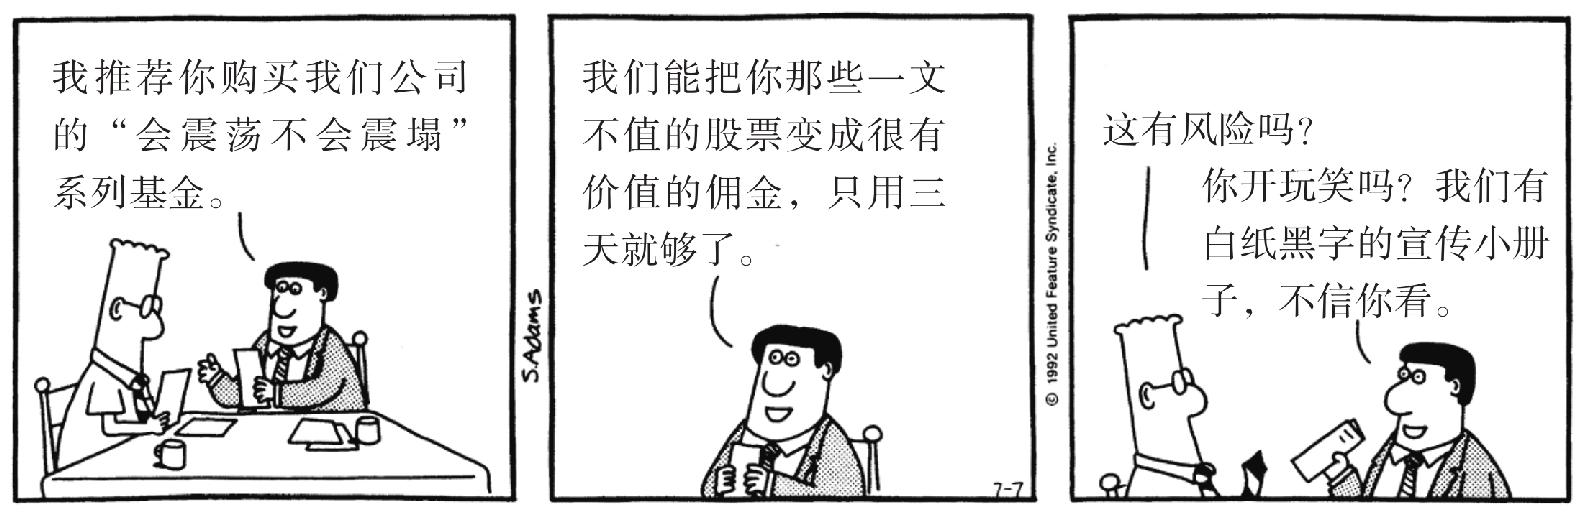
\includegraphics[width=0.98\linewidth,keepaspectratio]{image/7-2.jpg}
\caption{}\label{fig:7-2}
\end{figure}

\subsection{我比他们聪明多了}

你可能一边读一边想：“托尼，我比那家伙聪明多了，我看了我买的公募基金的费率，只有1\%。哈哈，我甚至还有‘免佣金基金’。”哦，是吗？我在佛罗里达州有块沼泽地想要卖给你！我要非常认真地说，这正是那些基金公司想要让你得出的结论。就像那些手法高超的魔术师一样，基金公司用的是最古老的手法：误导。它们希望我们能够专注地看着错误的目标，而它们却悄悄地拿走了我们的手表。费率其实就像是标签价格，基金公司都会在市场宣传材料上醒目地标识出来。但是标出来的费用并不是全部费用，只是一部分……

就让我来第一个公开承认吧。过去有段时间，我自认为自己在做聪明的投资，我持有的主动管理型基金都有五星评级。我事先做了很多功课。我仔细查看了基金的费率。我咨询了理财经理和证券公司经纪人。但是和你一样，我每天要忙着工作赚钱，照顾老婆孩子。我哪里有时间坐下来仔仔细细地阅读50页厚的基金招募说明书呢？里面的费用一览表隐藏在这些用极小字体印刷的招募说明书里。要把它们看明白，你得有经济学博士学位才行。

\subsection{研究基金费率的博士}

就在2008年股市大崩盘之后，罗伯特·希尔顿·史密斯博士研究生毕业了，他拿到了经济学博士学位，决定在一家政策智库大魔斯工作。跟大家一样，他在学校里学的东西并不能帮他搞定投资理财，他也不知道如何才能创立一个成功的投资策略。

于是，和我们大多数人一样，罗伯特·希尔顿·史密斯开始每个月尽心尽力地往401(k)账户里存钱。但是，尽管股市在上涨，他的账户却很少随着股市上涨。他知道肯定是哪里出错了，所以他决定把这件事作为自己的一个工作研究课题，好好研究一下。首先，他开始仔细阅读50页厚的基金招募说明书，他投资了20只基金，一份接一份地读那些招募说明书，它们读起来非常枯燥乏味，都是干巴巴的法律术语，用罗伯特·希尔顿·史密斯的话来说是“非常模糊”\footnote{\label{fn:pdf-7-2}罗伯特·希尔顿·史密斯和他的研究，后来被拍成一部很棒的纪录片《退休金大赌博》，2013年4月23日在美国公共广播公司纪录片频道首播。}。说明书里面有些表述像密码一样让他无法破译，有些首字母缩略语他根本猜不出来代表什么意思。更重要的是，说明书里面有收费目录表，列出了基金征收的17种不同的费用。另外还有一些附加成本，尽管不是直接收取费用，但是要转嫁到投资者身上，不用说，当然也要投资者来付钱。

为了更好地掩盖这些费用，华尔街和大多数401(k)计划供应商炮制出了五花八门且令人迷惑的专业术语：资本管理费、12b–1费（市场营销费）、交易成本（经纪人佣金、买卖价差成本、市场冲击成本）、非金钱利益成本、赎回费、开户费、申购费、保存记录费、规划管理费，等等。随便你用什么名字来称呼这些费用，本质上都一样。这些费用花的都是你的钱。你在攀登财务自由的山峰时，这些费用会把你往后拽。

做了一个月扎扎实实的研究，罗伯特·希尔顿·史密斯最后得出结论，他的401(k)账户根本不可能赚大钱，因为有这么多额外的费用和隐藏的费用，它们就好像在他坐的船上凿了一个洞。他后来写了一篇论文《吸干你的退休养老金：401(k)账户的隐藏成本和额外成本》。他计算出来，平均每个工作者一生要损失154794美元，这些钱都作为401(k)账户的费用让机构收走了（如此推算的依据是，年收入接近3万美元，且每年年收入储蓄率为5\%）。收入更高的工作者，每年收入约9万美元，这样最高会损失277000美元。罗伯特·希尔顿·史密斯和他所服务的智库大摩斯真是为整个社会做了一件大好事。他第一次揭露了这些费用长期按复利积累起来会给投资者造成多么巨大的损失。

\subsection{千刀万剐}

在古代中国，千刀万剐是最残酷的刑罚，因为要经过很长的过程，最后刽子手才会杀死犯人。现在遭受千刀万剐的就是美国投资者，传说中千刀万剐的刀刃就是过度征收的费用，慢慢地、稳稳地、一刀一刀地割掉投资者身上的肉，一滴一滴地放干投资者身上的血。

戴维·斯文森是耶鲁大学捐赠基金的投资主管，他把这只基金从10亿美元做到规模超过239亿美元，业内公认他就是机构投资界的沃伦·巴菲特，我专门去他在耶鲁大学的办公室拜访了他，跟他一起交流。我既受启发又非常愤怒，因为听到了他告诉我的事实真相，那些金融机构就像“费用工厂”一样制造出很多费用，像千刀万剐一样屠杀美国投资者。戴维·斯文森说：“非常普遍，公募基金从投资者那里榨取了巨额的财富。作为交换，它们给投资者提供的服务不仅无益，反而有害，非常有害。”在本书后面，我们会坐下来近距离仔细地倾听戴维·斯文森提出的投资组合建议，但是如果你让过多收取的费用一直在腐蚀你脚下的道路，那么不管你的投资策略多么伟大，它都没有用。

“资产收集”综合体和它们推销的主动管理型基金，在很大程度上，成了一场灾难性的社会实验，20世纪80年代早期引入的401(k)，就开始了这个实验。401(k)本身并不是一个“坏”的概念。对于那些想多存一些钱，让退休养老生活更好一些的人来说，这是一个好主意。但是401(k)本来只想成为传统退休养老金计划的一个补充，结果后来却成了主流。现在超过13万亿美元被投资到公募基金上，大多数基金都是401(k)账户和个人退休金账户持有的。投资者购买时以为这些基金能够战胜市场，但是不仅极少有基金能够战胜市场，而且很大一部分收费高得离谱，可业绩非常平庸。这些基金收费累计起来会让亿万投资者大幅降低生活品质。它很可能成为你财务自由的第一大危险和第一大杀手。我这样说，听起来是不是太夸张了？

先锋公司的创始人约翰·博格说：“我认为投资基金的成本过高（正在吞食本来已经很低的收益），这对投资者造成的危害程度是很大的。”

\subsection{真相/解决方案}

首先，你需要弄清楚你付的费用是多少钱。我推荐你使用网上的投资成本计算器，分析一下你持有的基金，了解你支付的费用比例是多少，以及其他成本。

记住，这些投资成本计算器只估计了费用，但根本不能准确地计算其他成本，比如税收，因为每个人的税率等级可能是不同的。你持有的基金，也许是在你的401(k)账户里持有的，你的基金投资增值根本不用交税，但是你要付一笔“计划管理费”。有些401(k)计划是低成本的，而有些401(k)计划的成本非常高。平均而言，计划管理人每年要收取1.3\%\textasciitilde{}1.5\%的管理费（这是中立机构美国政府问责局的研究结论）。也就是说，我们为了参加401(k)计划，每投资10万美元就要拿出来1300美元左右作为管理费。所以当你把这1.3\%的计划管理费加上公募基金的管理费3.17\%时，你支付的管理费高达4.47\%，结果实际上你用一个免税账户来持有一只基金，比用一个需要交税的投资账户投资一只基金，实际所需要付的费用更高（每年的费用比例高达4.47\%\textasciitilde{}4.67\%）。

好好想想：你辛辛苦苦赚钱又想方设法地省钱，才储蓄下来年收入的10\%，但是其中一半要付给机构。这也太荒唐了吧？不过，读到这里你会明白，你根本不用让自己掉进这个深坑，让基金坑你。你跟我学习进步，成了投资内行，你就会对基金这些过度收费的行为大声喊停。承受如此高昂的费用，相当于你在攀登珠穆朗玛峰时，穿着人字拖和短裤背心。你还没有开始爬山，就会被冻死。

% 来源：OEBPS/Text/Section0001_split_002.xhtml → image_7173dd9591614bfab3dc9499b2a05449.jpg
\begin{longtable}{@{}C{\dimexpr 0.50000\linewidth-1.00000\tabcolsep\relax}C{\dimexpr 0.50000\linewidth-1.00000\tabcolsep\relax}@{}}
\caption{持有一只基金的真实成本}\label{tab:7-1}\\
\toprule\noalign{\vskip 3pt}
{\heiti 免税账户} & {\heiti 纳税账户} \\
\midrule
\endfirsthead
\multicolumn{2}{r}{续表}\\[0.6em]
\toprule\noalign{\vskip 3pt}
{\heiti 免税账户} & {\heiti 纳税账户} \\
\midrule
\endhead
\bottomrule
\endfoot
\bottomrule
\multicolumn{2}{@{}p{\linewidth}@{}}{\footnotesize 基金费用合计。 资料来源：《福布斯》杂志，2011年4月4日}\\
\endlastfoot
费率，0.90\% & 费率，0.90\% \\
交易成本，1.44\% & 交易成本，1.44\% \\
现金拖累，0.83\% & 现金拖累，0.83\% \\
—— & 税收成本，1.00\% \\
总成本，3.17\% & 总成本，4.17\% \\
\end{longtable}


\begin{figure}[htbp]
\centering
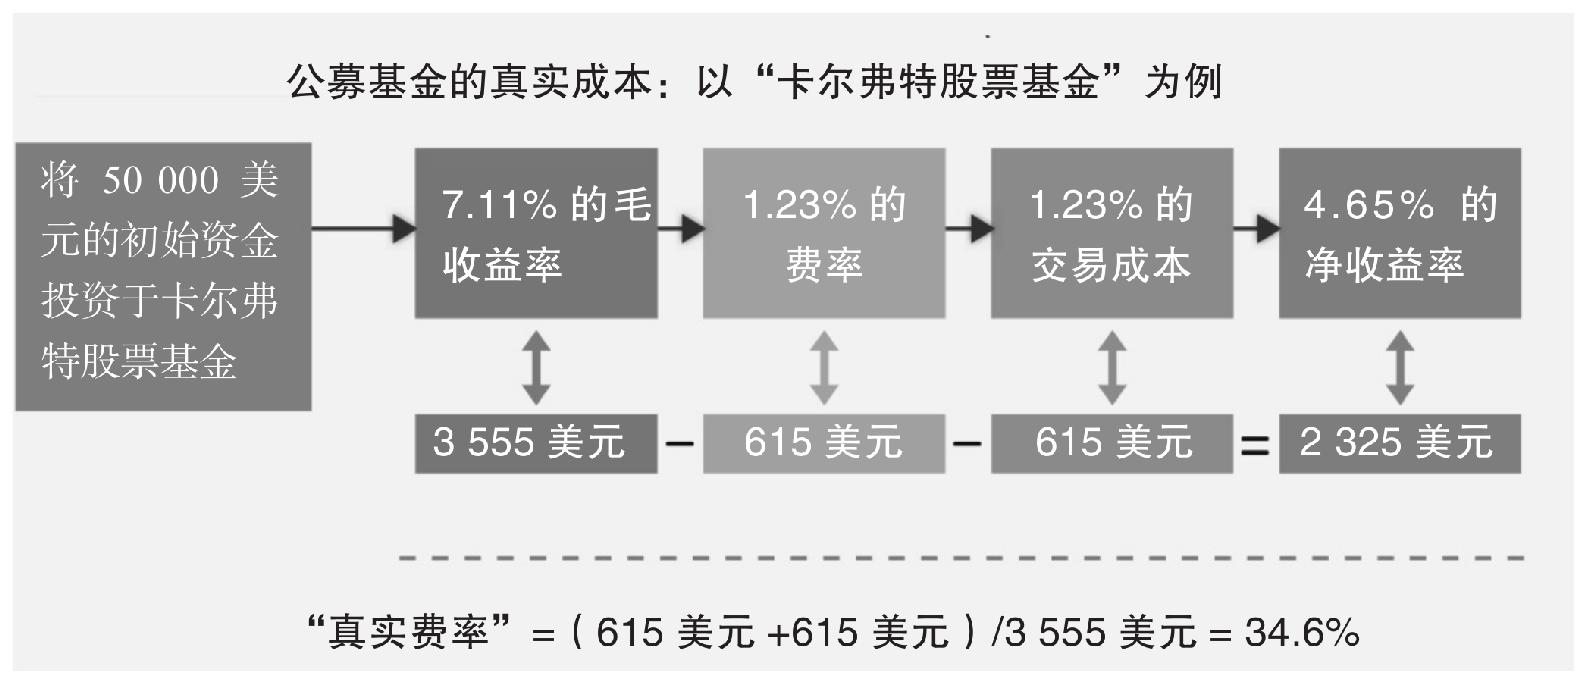
\includegraphics[width=0.98\linewidth,keepaspectratio]{image/7-3.jpg}
\caption{}\label{fig:7-3}
\end{figure}

\subsection{逃离}

要逃离这些专门制造费用的工厂，你必须降低你的整体年度费率和相关的投资成本，降到1.25\%，甚至更低的平均水平。这意味着你获得投资建议的成本（请一个注册投资顾问来帮助你合理配置资产，定期进行再平衡投资组合，等等），加上投资的成本，理想情况下应该是1.25\%，或者更低。例如，你需要支付1\%左右的费用给注册投资顾问，0.2\%的管理费给一只低成本的指数基金，就像先锋公司提供的那些指数基金一样，这样投资费用总计为1.2\%。而且付给注册投资顾问的1\%的费用是可以抵税的。这意味着从你口袋里拿出来的“净”成本少了接近一半，当然具体能扣多少税，取决于你的个人所得税的税率等级。大多数美国人的基金经纪人，他们的佣金是不能抵税的，公募基金收取的那些昂贵费用也是不能抵税的。（我们后面会讨论经纪人和注册投资顾问的区别。你一定不要错过这个部分。）

在第三部分我会演示给你看，如何一步一步地大幅削减你的费用，合法减少你的税款。你省下来的所有钱，都会加快你实现财务自由的速度。

\subsection{永远不要重蹈覆辙}

现在你已经知道这个游戏是怎么玩的了，你也看到了幕后的真相，你应该做出决定，以后再也不要让人利用了。现在就下定决心，你再也不会是任人宰割的“绵羊投资者”中的一个了。现在你成了投资内行了。你不再是让人玩弄的棋子，而是一个会玩弄棋子的棋手。知识就是力量，但是执行力远远胜过知识的力量。因此，真正重要的是从现在开始你会做什么。是的，我将会向你展示具体如何操作来减少你的费用，但是必须由你本人来决定是否采取必要的行动。你必须声明，你再也不会给那些业绩低于市场平均水平的基金支付高于市场平均水平的费用。如果本书能够每年让你省下来2\%\textasciitilde{}3\%不必要的费用，那我们就相当于把成千上万的现金，甚至是数百万的现金，重新装回到你的口袋里。换句话说，这些钱会让你更快地实现你的目标，为你节省5\textasciitilde{}15年的财富积累时间，让你可以随自己的意愿决定是否提前退休。

只要简单地抛弃那些收费昂贵的公募基金，替换成低成本的指数基金，你就迈出了一大步，重新拿回来了70\%的未来投资收益，这让你的养老金大幅增长！这多让人心动啊！这对你和你的家庭的意义会是多么重大啊！先锋公司全套的低成本指数基金（各种各样的资产类型都有），每年所有的成本加在一起也只有0.05\%\textasciitilde{}0.25\%。三维基金顾问公司是另外一个伟大的低成本指数基金提供商。如果你的401(k)计划基金投资选项不包括这些提供低成本指数基金的基金公司，我们会展示给你如何操作就能买到这两家公司的指数基金。低成本指数基金至关重要，但决定每只指数基金买多少，如何长期管理整个投资组合也非常重要，这三点是投资成功的关键。我们会在后面详细讨论。

现在既然你下定决心要采取行动，那么你去向谁求助呢？谁值得你信任，可以当你的向导呢？回过头去找你的经纪人和理财经理来帮助你节省费用，就像是你去找你的药剂师来帮助你摆脱药物一样，那是根本不可能的。你怎样才能找到没有利益冲突的投资建议？你如何能知道自己得到的投资指导，并不是让桌子那头指导你投资理财的那个人自己的利益最大化？现在翻到下一章，我们来揭开第3个投资营销谎言，让我们找到答案来解决这些紧迫的问题……

\subsection{详解基金成本费用}

你如果真的想知道那些隐藏费用把你害得多么惨，拿出点时间仔细看看下面核心费用和成本的详解，看看它们对你的公募基金的投资影响有多大。

1.费率。这种费用是主要的标签价格——那些基金公司想让我们只把目光聚焦在这些费用上，但是费用肯定不只这些。根据晨星公司的研究，美国股票基金每年平均要拿出资产的1.31\%，付给基金公司作为投资组合的管理费用和运营费用，比如市场营销费（12b–1费）、市场分销费、行政管理费。很多规模比较大的基金已经意识到，它们收取的费用整体要保持在1\%左右，好让投资者不会一看就害怕，也让那些银行理财经理和证券经纪人有好的故事可以卖——我的意思是忽悠人。

2.交易成本。交易成本是个范围很广的普遍费用类型，并可以进一步分解成很多更细的类型，比如，券商佣金、市场冲击成本（基金大规模交易对市场价格形成反向冲击，导致无法按照目标价格交易，从而产生的成本）、买卖价差成本（买入报价和卖出报价之间的价差，或者买入价格和卖出价格之间的价差）。2006年，由三位商学院教授罗杰·艾德伦、格雷格·卡德莱茨、理查德·埃文斯撰写的研究报告发现，美国股票类公募基金平均每年的交易成本约为1.44\%，这意味着这些交易成本可能是持有一只公募基金最大的成本，但是业内认为交易成本太难被量化，因此公募基金公开披露的文件中并不报告这项费用。

3.税收成本［401(k)成本］。很多人都很激动，因为用401(k)账户投资能够得到递延纳税的优惠待遇，但是对于大多数雇员来说，税收成本只不过换成了账户计划管理费。很多人不知道，用401(k)账户投资基金，你除了要支付管理费等费用外，还要向账户管理人支付一笔计划管理费。根据中立机构政府问责局的研究，401(k)计划管理费平均每年为1.13\%。如果你持有一只公募基金，用的是需要纳税的投资账户，平均税收成本每年在1.0\%\textasciitilde{}1.2\%，这是晨星公司的统计数据。由此可以看出，二者成本基本相当。

4.非金钱利益成本。非金钱利益交易是一种利益交换，公募基金管理人选择支付过度膨胀的证券交易成本，好让执行这些证券交易的外部证券公司多支付的那些成本返给基金经理，业内俗称返佣。其实这是使用某个券商交易通道的奖励计划。华尔街证券公司模仿航空公司搞的常旅客飞行里程累积计划，允许用这些“积分”来支付某些特定的费用，比如购买研究报告。不然的话，基金公司就得花钱（真金白银）购买。最终的结果都是一样的，都由我们这些基金投资人来买单。这些其实都是基金公司伪装得很好的提高管理费收入的手段，最终增加的是基金公司的利润。这些非金钱利益成本根本不会公开披露，而且几乎不可能量化，所以也根本无法纳入我们计算基金投资成本的公式。但是不要忽略，这些确确实实是成本。

5.现金拖累。公募基金必须保持一定的现金头寸，以保证日常的流动性，满足任何种类的基金赎回（基民卖出基金）。保留现金意味着不能用这些钱来投资，也就不能产生投资收益。因此，现金会拖累基金业绩表现。有一份研究报告《如何做好主动投资》，它的作者是威廉·奥赖利和迈克·朴尔萨诺，其研究结果表明，大盘股基金的现金拖累造成的平均成本，按照十年期限估算，平均每年为0.83\%。这尽管不是一项直接的费用，但是确实是一项投资成本，它又从你本来能够得到的投资业绩中拿走了一部分。

6.赎回费。如果想卖出你持有的基金，你必须支付一笔赎回费。赎回费直接付给基金公司。美国证券交易监督委员会限定赎回费最高不超过2\%。这就像是世界上最昂贵的自动取款机，你要取回自己的10万美元，要付2000美元的取现费。

7.转换费。如果你从一只基金转换到另外一只基金，尽管两只基金都是同一家基金公司旗下的基金，但是公司还是要收取你一笔转换费。

8.账户维护费。有些基金要收取你一笔维护费，只是让你能有一个账户。

9.申购费。不要把申购费跟前端的销售手续费（佣金）混为一谈，这个申购费是你购买基金时直接支付给基金公司的。（中国国内首发基金称之为认购费。）

10.手续费（佣金）或者递延销售佣金。这项收费是付给经纪人或银行理财经理的，要么在你购买基金时支付，要么在你退出基金，赎回你持有的基金份额时支付。
